\begin{solution}
  متغیر $ r = \frac{x}{y}$ را برای متغیرهای تصادفی انتخاب‌شده $ x $ و $ y $ تعریف کنیم. همچنین تابع احتمال $ f(a,b) $ را به صورت زیر تعریف می‌کنیم:

$$ f(a,b) = \mathsf{Pr}(a \leq r \leq b). $$

با این تعریف، پاسخ مسئله برابر با $ f(0,0.5) + f(1.5, 2.5) + f(3.5, 4.5) + \ldots $ خواهد بود. بنابراین، پاسخ نیاز به تعیین مقدار تابع $ f(a,b) $ بستگی دارد. به این منظور، دو حالت را به طور جداگانه بررسی می‌کنیم: 
1. هر دو $ a $ و $ b $ کوچکتر از 1 باشند.
2. هر دو $ a $ و $ b $ بزرگتر از 1 باشند.

حالت (i): هر دو $ a $ و $ b $ کوچکتر از 1 هستند: در این صورت، یک نقطه $ p = (x, y) $ را در نظر بگیرید که مختصات آن برابر با $ x $ و $ y $ هستند. این نقطه در یک مربع واحد قرار دارد که نقاطی با مختصات بین 0 و 1 را پوشش می‌دهد. با این حال، $ \frac{x}{y} $ در بازه $ [a, b] $ قرار خواهد گرفت اگر و فقط اگر نقطه روی مثلثی باشد که توسط دو پیکان ساخته شده است. از آنجایی که مساحت مثلث برابر با $ \frac{b-a}{2} $ است و مساحت مربع برابر با 1 می‌باشد، احتمال اینکه $ a \leq \frac{x}{y} \leq b $ برقرار باشد برابر با $ \frac{b-a}{2} $ خواهد بود.

\begin{center}
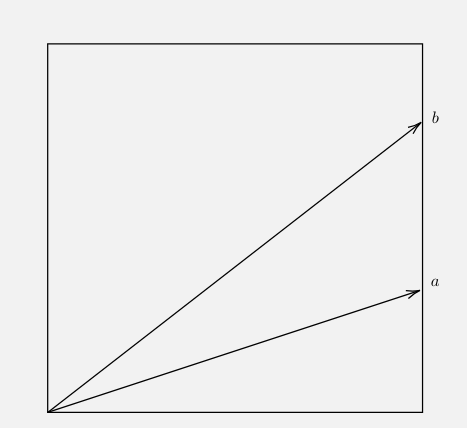
\includegraphics[width=\textwidth]{/images/problems/83_sol.png}
\end{center}
حالت (ii): هر دو $ a $ و $ b $ بزرگتر از 1 هستند. این حالت نیز مشابه حالت قبلی است، با این تفاوت که نسبت $ \frac{x}{y} $ تنها در صورتی بین $ a $ و $ b $ قرار می‌گیرد که نقطه $ p $ روی مثلث نشان داده‌شده در شکل زیر باشد. توجه داشته باشید که مساحت این مثلث برابر با $ \frac{1/a - 1/b}{2} $ است. بنابراین، احتمال اینکه $ \frac{x}{y} $ بین $ a $ و $ b $ باشد نیز برابر با $ \frac{1/a - 1/b}{2} $ خواهد بود.
\begin{center}
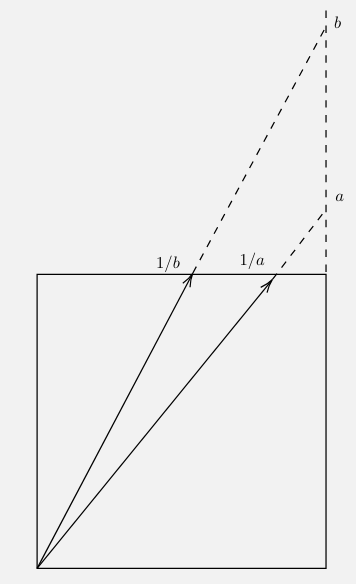
\includegraphics[width=\textwidth]{/images/problems/83_sol2.png}
\end{center}
بر اساس استدلال‌های فوق، پاسخ مسئله برابر است با 
\begin{align}
f(0,0.5) + \sum_{i=1}^{\infty} f(2i-0.5, 2i+0.5)  &= 0.25 + \sum_{i=1}^{\infty}  \frac{1/(2i-0.5) - 1/(2i+0.5)}{2} \nonumber  \\
& = 0.25 + \sum_{i=1}^{\infty}  (1/(4i-1) - 1/(4i+1)) \nonumber \\
& = 0.25 + \sum_{i=2}^{\infty}  (-1)^i/(2i-1) \nonumber  \\
& = 0.25 + 1-\pi/4 \label{eq:one}\\
& = 1.25-\pi/4 \nonumber
\end{align}
 که از فرمول لایبنیتس ($ \pi/4 = 1 - 1/3 + 1/5 - 1/7 \ldots $) استفاده کرده‌ایم.
\end{solution}
